\documentclass[a4paper]{article}
\usepackage{a4wide}
\usepackage{amsmath}
\usepackage{amsfonts}
  \DeclareMathOperator*{\argmax}{arg\,max}
  \newcommand{\ex}[1]{{\mathbb E}\left[ #1 \right]}
  \newcommand\norm[1]{\left\lVert#1\right\rVert}
\usepackage{booktabs}
\usepackage{csquotes}
\usepackage{upquote}
\usepackage{float}
\usepackage{graphicx}
\usepackage{enumerate}
\usepackage{subcaption}
\usepackage{xcolor}


\title{Pattern and Speech Recognition WS2015-16 \\ Exercise 4}
\author{Atanas Poibrenski(2554135), Marimuthu Kalimuthu(2557695), Furkat Kochkarov(2557017)}

\begin{document}

\maketitle
\section*{Probability Theory}

\begin{enumerate}
	\item A,B $->$ two events \newline
	
	P(A).P(B) = $P(A \cap B)$ ; $P(A|B)$  = P(A)
	
	Yes they are equivalent, since independence is assumed.
	
	\begin{align*}
			P(A \cap B) & = P(A,B) \\
			& = P(A).P(B|A) \\
			\intertext{If A \& B are independent,}
			& = P(A).P(B) \\
			\intertext{Also}
			\boxed{P(A|B) = P(A)} \\
	\end{align*}
		
\item Bayes Law \newline
	\begin{align*}
		P(A \cap B) & = P(A).P(B|A) \\
		& = P(B).P(A|B) \\
		P(A|B) & = \frac{P(B|A)P(A)}{P(B)}
		\intertext{which is Bayes law.}
	\end{align*}

\item \textbf{Bonus:} \newline
	\begin{align*}
		\ex{X+Y} = \ex{X} + \ex{Y} \\
		\ex{X} & = \int_{-\infty}^{\infty}xf(x) dx \\
               & = \frac{1}{\sigma\sqrt{2\pi}} \int_{-\infty}^{\infty}x e^{\frac{-(x-\mu)^2}{2\sigma^2}} dx \\
               & = \frac{1}{\sigma\sqrt{2\pi}} \int_{-\infty}^{0}x e^{\frac{-(x-\mu)^2}{2\sigma^2}} dx +
               \frac{1}{\sigma\sqrt{2\pi}} \int_{0}^{\infty}x e^{\frac{-(x-\mu)^2}{2\sigma^2}} dx \\
               & = \mu
              \intertext{similarly for}
              \ex{Y} & = \mu \\
       		\boxed{ \ex{X+Y}  = 2\mu } \\
	\end{align*}
	
	$Var[X+Y] = Var[X] + Var[Y]$
	\begin{align*} \\
		Var[X] & = \ex{(x-\mu)^2} \\
		\ex{(x-\mu)^2} & = \int_{-\infty}^{\infty} (x-\mu)^2 f(x)dx \\
		&= \frac{1}{\sqrt{2\pi}\sigma} \int_{-\infty}^{\infty} (x-\mu)^2 e^{\frac{-(x-\mu)^2}{2\sigma^2}} dx \\
		\intertext{on evaluating the integral, we get}
		& = 0 + \sigma^2.1 \\
		& = \sigma^2
		\intertext{similarly,}
		Var[Y] & = \sigma^2 \\
		\intertext{Hence,}
		\boxed{Var[X+Y]  = 2 \sigma^2}
	\end{align*}

\end{enumerate}


\section*{MLE for Poisson Distribution}

\begin{enumerate}
	\item Likelihood

\begin{align*}
	L(\theta; k) & = \prod_{i=1}^{n} \frac{e^{-\theta}\theta^{k_{i}}}{k_{i}!} \\
	& = e^{-n\theta}\theta 
\end{align*}
\newpage
See `poisson\_likelihood.m'

	\begin{figure}[H]
		\begin{center}
			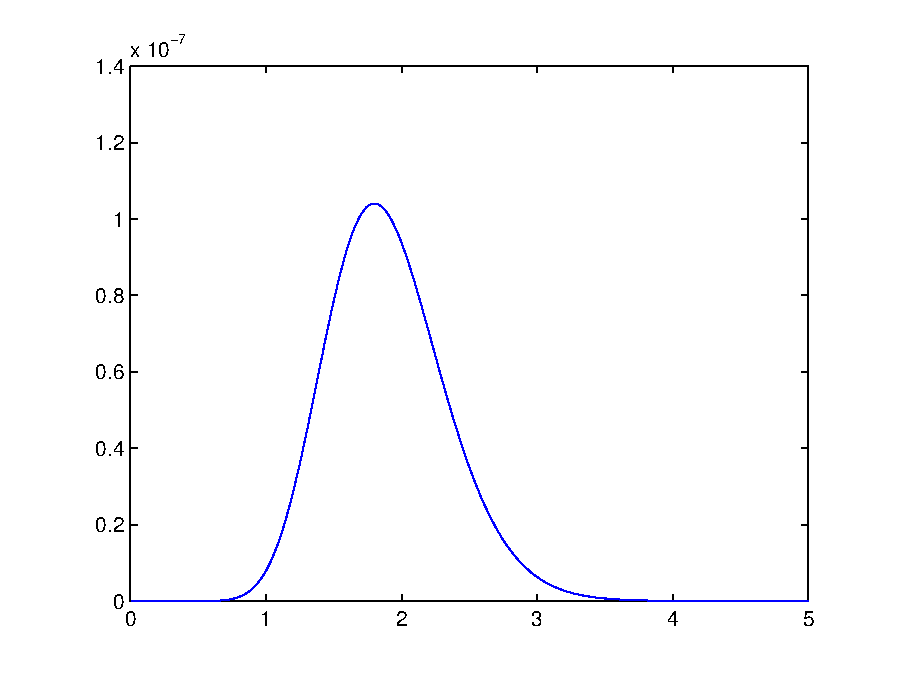
\includegraphics[width=0.80\textwidth]{poisson_likelihood.eps}
			\caption{Poisson likelihood (for $\theta \in (0,5]$)}\label{fig:poissonlh}		
		\end{center}
	\end{figure}

\item See `poisson\_loglikelihood.m'
	\begin{figure}[H]
		\begin{center}
			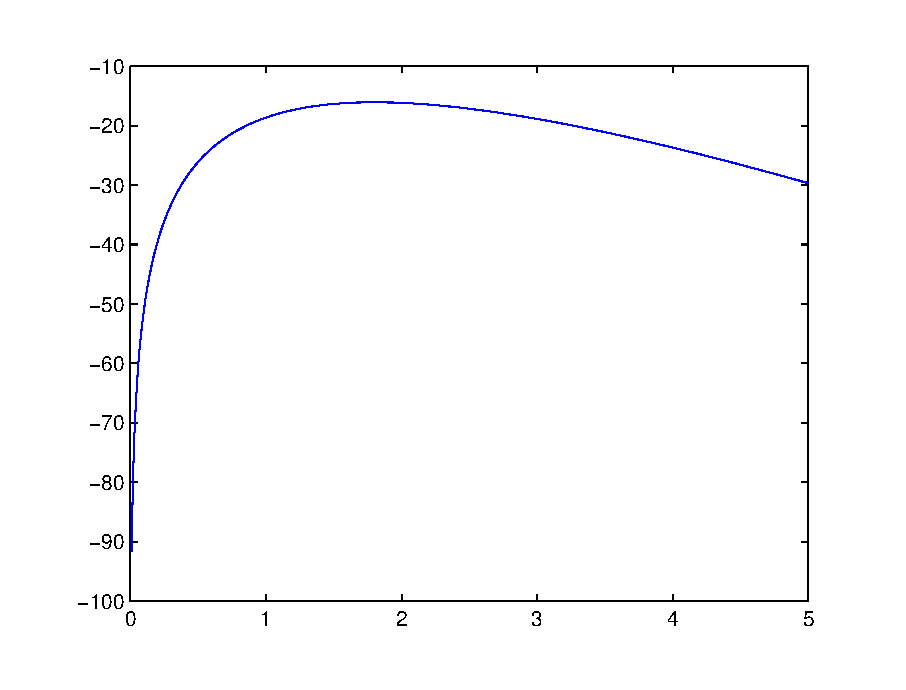
\includegraphics[width=0.80\textwidth]{poisson_loglikelihood.eps}
			\caption{Poisson log-likelihood (for $\theta \in (0,5]$)}\label{fig:poissonllh}		
		\end{center}
	\end{figure}

Here we notice that since log is a monotonically increasing function, it achieves maximum at the same $\theta$ as in the likelihood plot. So, we can use either of them to find the maximum.

\item Here we use log-likelihood

\begin{align*}
	L(\theta|x) = \sum_{i=1}^{n} (x_{i} ln\theta) - n\theta \\
	\frac{\partial L(\theta | x)}{\partial \theta} = 0 \\ \newline
	\frac{\sum_{i=1}^{n}x_{i}}{\theta} - n  = 0 \\
	\theta_{max}  =  \frac{\sum_{i=1}^{n}x_{i}}{n} \\
	\intertext{In our case, x=0,2,2,1,2,1,3,1,1,5}
	\boxed{\theta_{max}  =  1.8}
\end{align*}
\end{enumerate}



\section*{MLE for Normal Distribution}
\begin{enumerate}
	\item After importing Iris-setosa, Iris-versicolor, we get the following 1-D plot (histogram)
	
	\begin{figure}[H]
		\begin{center}
			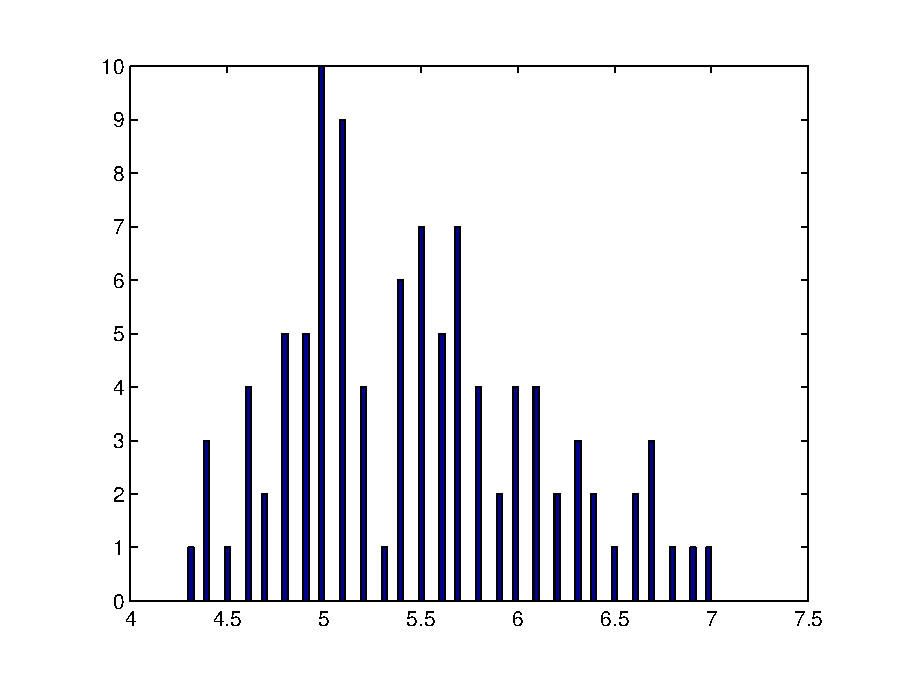
\includegraphics[width=0.89\textwidth]{iris_dataset.eps}
			\caption{ Iris-setosa and Iris-versicolor} \label{fig:irisdata}
		\end{center}
	\end{figure}
	
	\item Maximize the likelihood
	\begin{align*}
		p_{\theta}(x_{i}) = \frac{1}{b-a} \hspace*{2em} if (a\le x_{i} \le b) \\
		\intertext{To maximize $p_{\theta}(x_{i})$ we need to minimize (b-a). The smallest interval which contains all the points. That is a=min(x) and b=max(x)}.
		\intertext{In the case of the Iris dataset, a=4.3 and b=7}	
	\end{align*}

	\item $p_{\theta}$ is a probability density. \newline
	$p_{\theta}(x_{i}) = \frac{1}{2} . f_{\mu_{1}, \sigma{1}}(x_{i}) + \frac{1}{2}. f_{\mu_{2}, \sigma{2}}(x_{i}) $  \\ \newline
	The normal distribution is a probability density because $\int p(x) dx = 1$ \\
	$p_{\theta}$ is a probability density because, \newline
	
	 $ => \frac{1}{2}.1 + \frac{1}{2}.1 = 1 $
	 
	 \item See `normal\_likelihood.m' and `normal\_loglikelihood.m' \newline
	 We prefer log-likelihood since it is numerically stable. Since the likelihood gives very small probabilities ( Figure \ref{fig:poissonlh}), it is easier to compute and represent log-likelihood where the product becomes summation.
	 
	 \item We use log-likelihood to estimate the parameter $\theta_{max}$ for the reason stated above. We used `fminsearch' in matlab with the initial guess(6.0, 0.6, 5.0, 0.5) in order to find  \\
	 $\theta_{max} = [5.47, 0.63, 5.25, 0.5]$ 
	 
	 	\begin{figure}[H]
	 		\begin{center}
	 			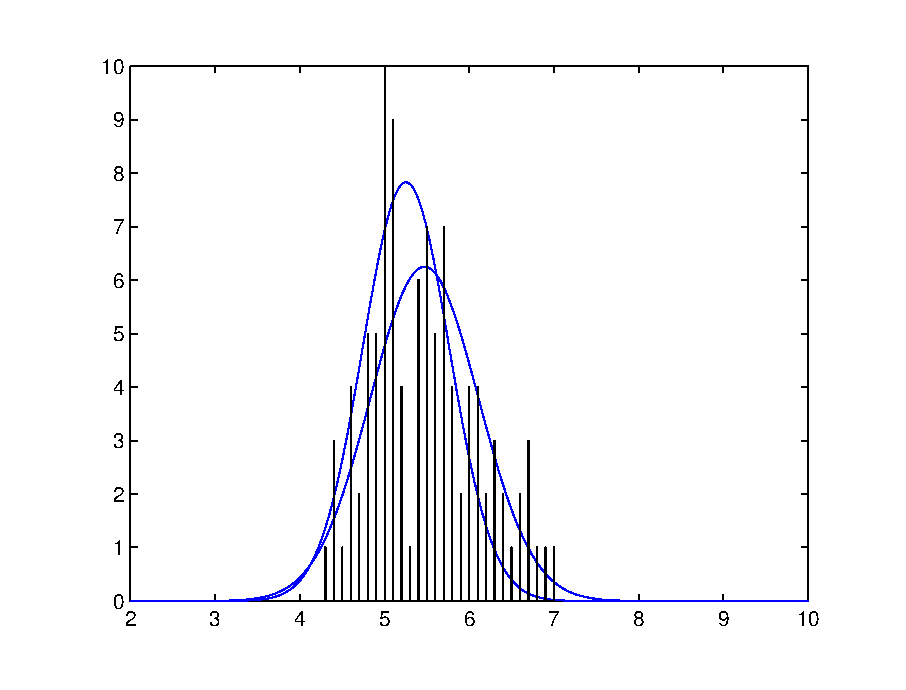
\includegraphics[width=0.89\textwidth]{normal_distributions.eps}
	 			\caption{ Normal distribution} \label{fig:normdist}
	 		\end{center}
	 	\end{figure}
	 
	 See `drawgaussian.m'
	 
\end{enumerate}

\end{document}
